The ``i2ctools'' detect commands listed in Section \ref{I2Cdisc} were used to
list the connected I2C busses, and to show the devices connected to the busses.
From the screenshot shown in Figure \ref{fig:images-i2cDetect} it can be seen
that the RTC was installed on bus 1 (i2c-1), and had an address of 0x68.

\begin{figure}[H]
	\centering
	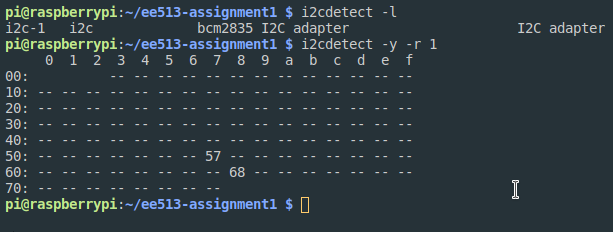
\includegraphics[width=0.8\textwidth]{images/i2cDetect}
	\caption{I2C Detect Output}
	\label{fig:images-i2cDetect}
\end{figure}

The dump command, also listed in Section \ref{I2Cdisc} was used to show the
values stored in the RTC registers. Registers 0x00 to 0x12 contain the time,
date, alarm, temperature and control registers. The values contained in these
registers can be seen in Figure \ref{fig:images-i2cDump}.

\begin{figure}[H]
	\centering
	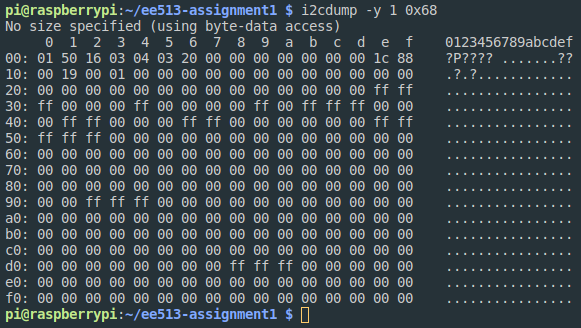
\includegraphics[width=0.8\textwidth]{images/i2cDump}
	\caption{I2C Dump Output}
	\label{fig:images-i2cDump}
\end{figure}

In order to verify the execution of the code, a test script was written.
This script contains the necessary function calls to test the required
functionality for this assignment. Before executing the test executable, the
novel function is run (using the main.cpp file). This sets the time on the RTC
to the initial value read in Figure \ref{fig:images-testing}.

\begin{figure}[H]
	\centering
	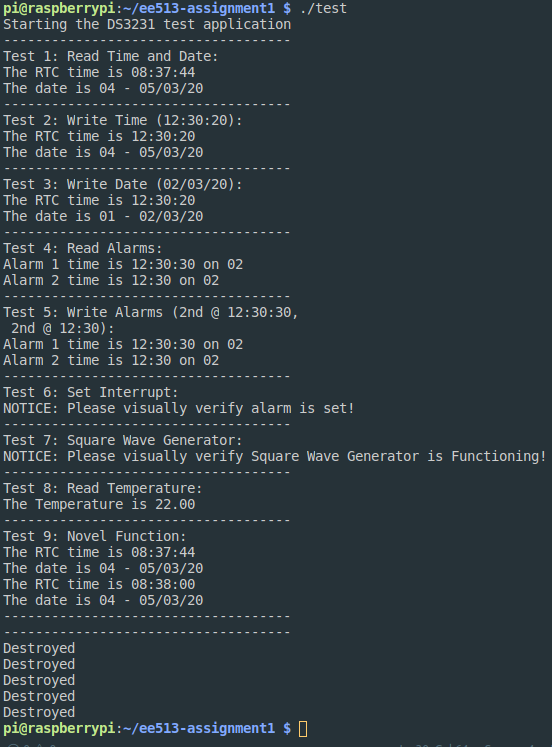
\includegraphics[width=0.8\textwidth]{images/testing}
	\caption{Testing Output}
	\label{fig:images-testing}
\end{figure}

The test scripts divides the required functionality into a number of tests. One
``DS3231'' object executes all of the write functions, with a new object
required for each of the subsequent read functions. This is due to the read
function reading from the initially stored buffer values.

\subsubsection{Test 1: Read Time and Date}

As mentioned previously, the initial time read from the RTC was set via the
novel function i.e. the system clock time. The output of this test shows the
time and date are being read correctly from the RTC.

\subsubsection{Test 2: Write Time}

The time being written to the registers is 12:30:20, i.e. 12 hours, 30 minutes,
and 20 seconds. The read function verifies that this time is being correctly
written to the registers. An hour value of greater than 9 was used to verify
that the upper nibble of data was not being unintentionally modified, with only
the desired bits being changed.

\subsubsection{Test 3: Write Date}

The date being written to the registers is 02/03/2020, with the day of the week
set to 1. Again the read function is used to verify this change. It can be seen
from Figure \ref{fig:images-testing} that the date has changed to the input
value.

\subsubsection{Test 4: Read Alarms}

The read alarm function output shows the values which are stored in the alarm
registers. These values are set from a previous execution of the test script.

\subsubsection{Test 5: Write Alarms}

The time and date being written to the alarm registers are 12:30:30 on the
2$^{nd}$ for Alarm 1 and 12:30 on the  $2^{nd}$ for Alarm 2. As these values
were written on a previous execution, there is no change to the register, as is
expected.

\subsubsection{Test 6: Set Interrupt}

The set interrupt function allows for the alarm flag to trigger the interrupt on
the square wave output. A delay in the code allows the user to verify that the
interrupt is triggered. The alarm flag being raised causes the interrupt output
to stop, i.e. the LED being used for visual verification turning off. This can
be seen in the following images, the first showing that the LED is lit before
the alarm condition is met, and the second showing the LED is not lit after the
alarm condition is met.

\begin{figure}[H]
	\centering
	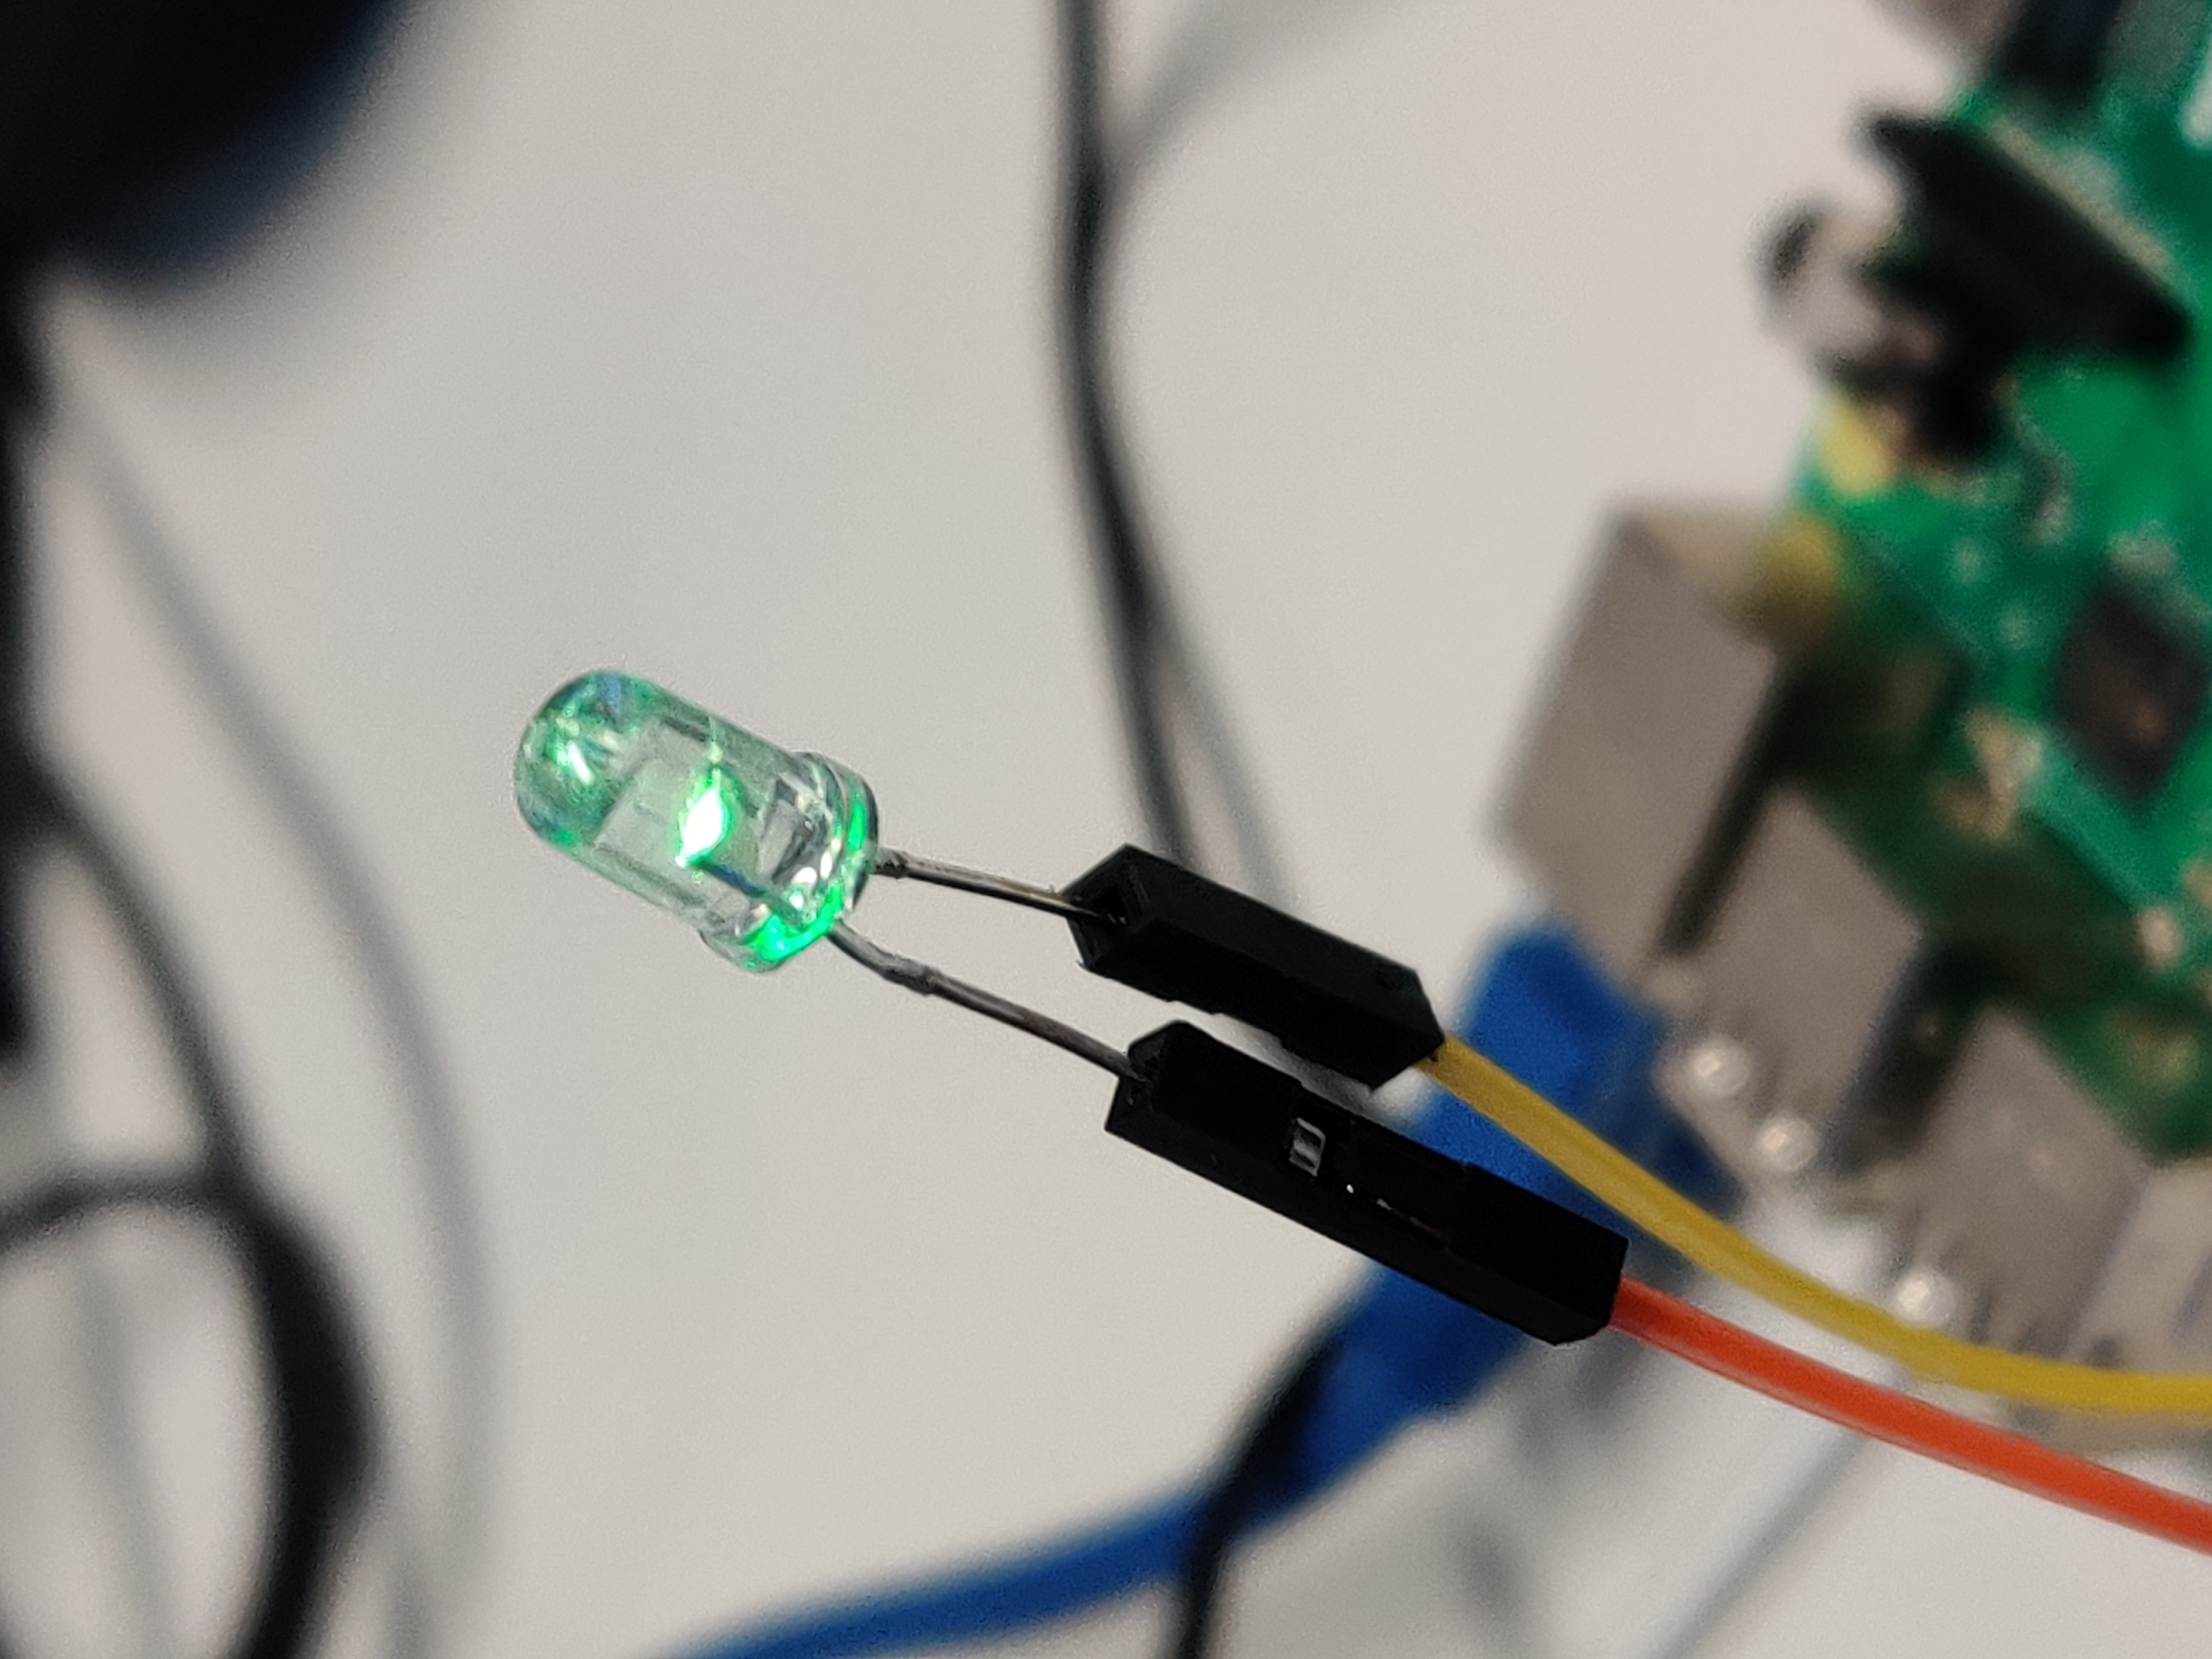
\includegraphics[width=0.8\textwidth]{images/ledOn}
	\caption{LED before alarm condition}
	\label{fig:images-ledOn}
\end{figure}

\begin{figure}[H]
	\centering
	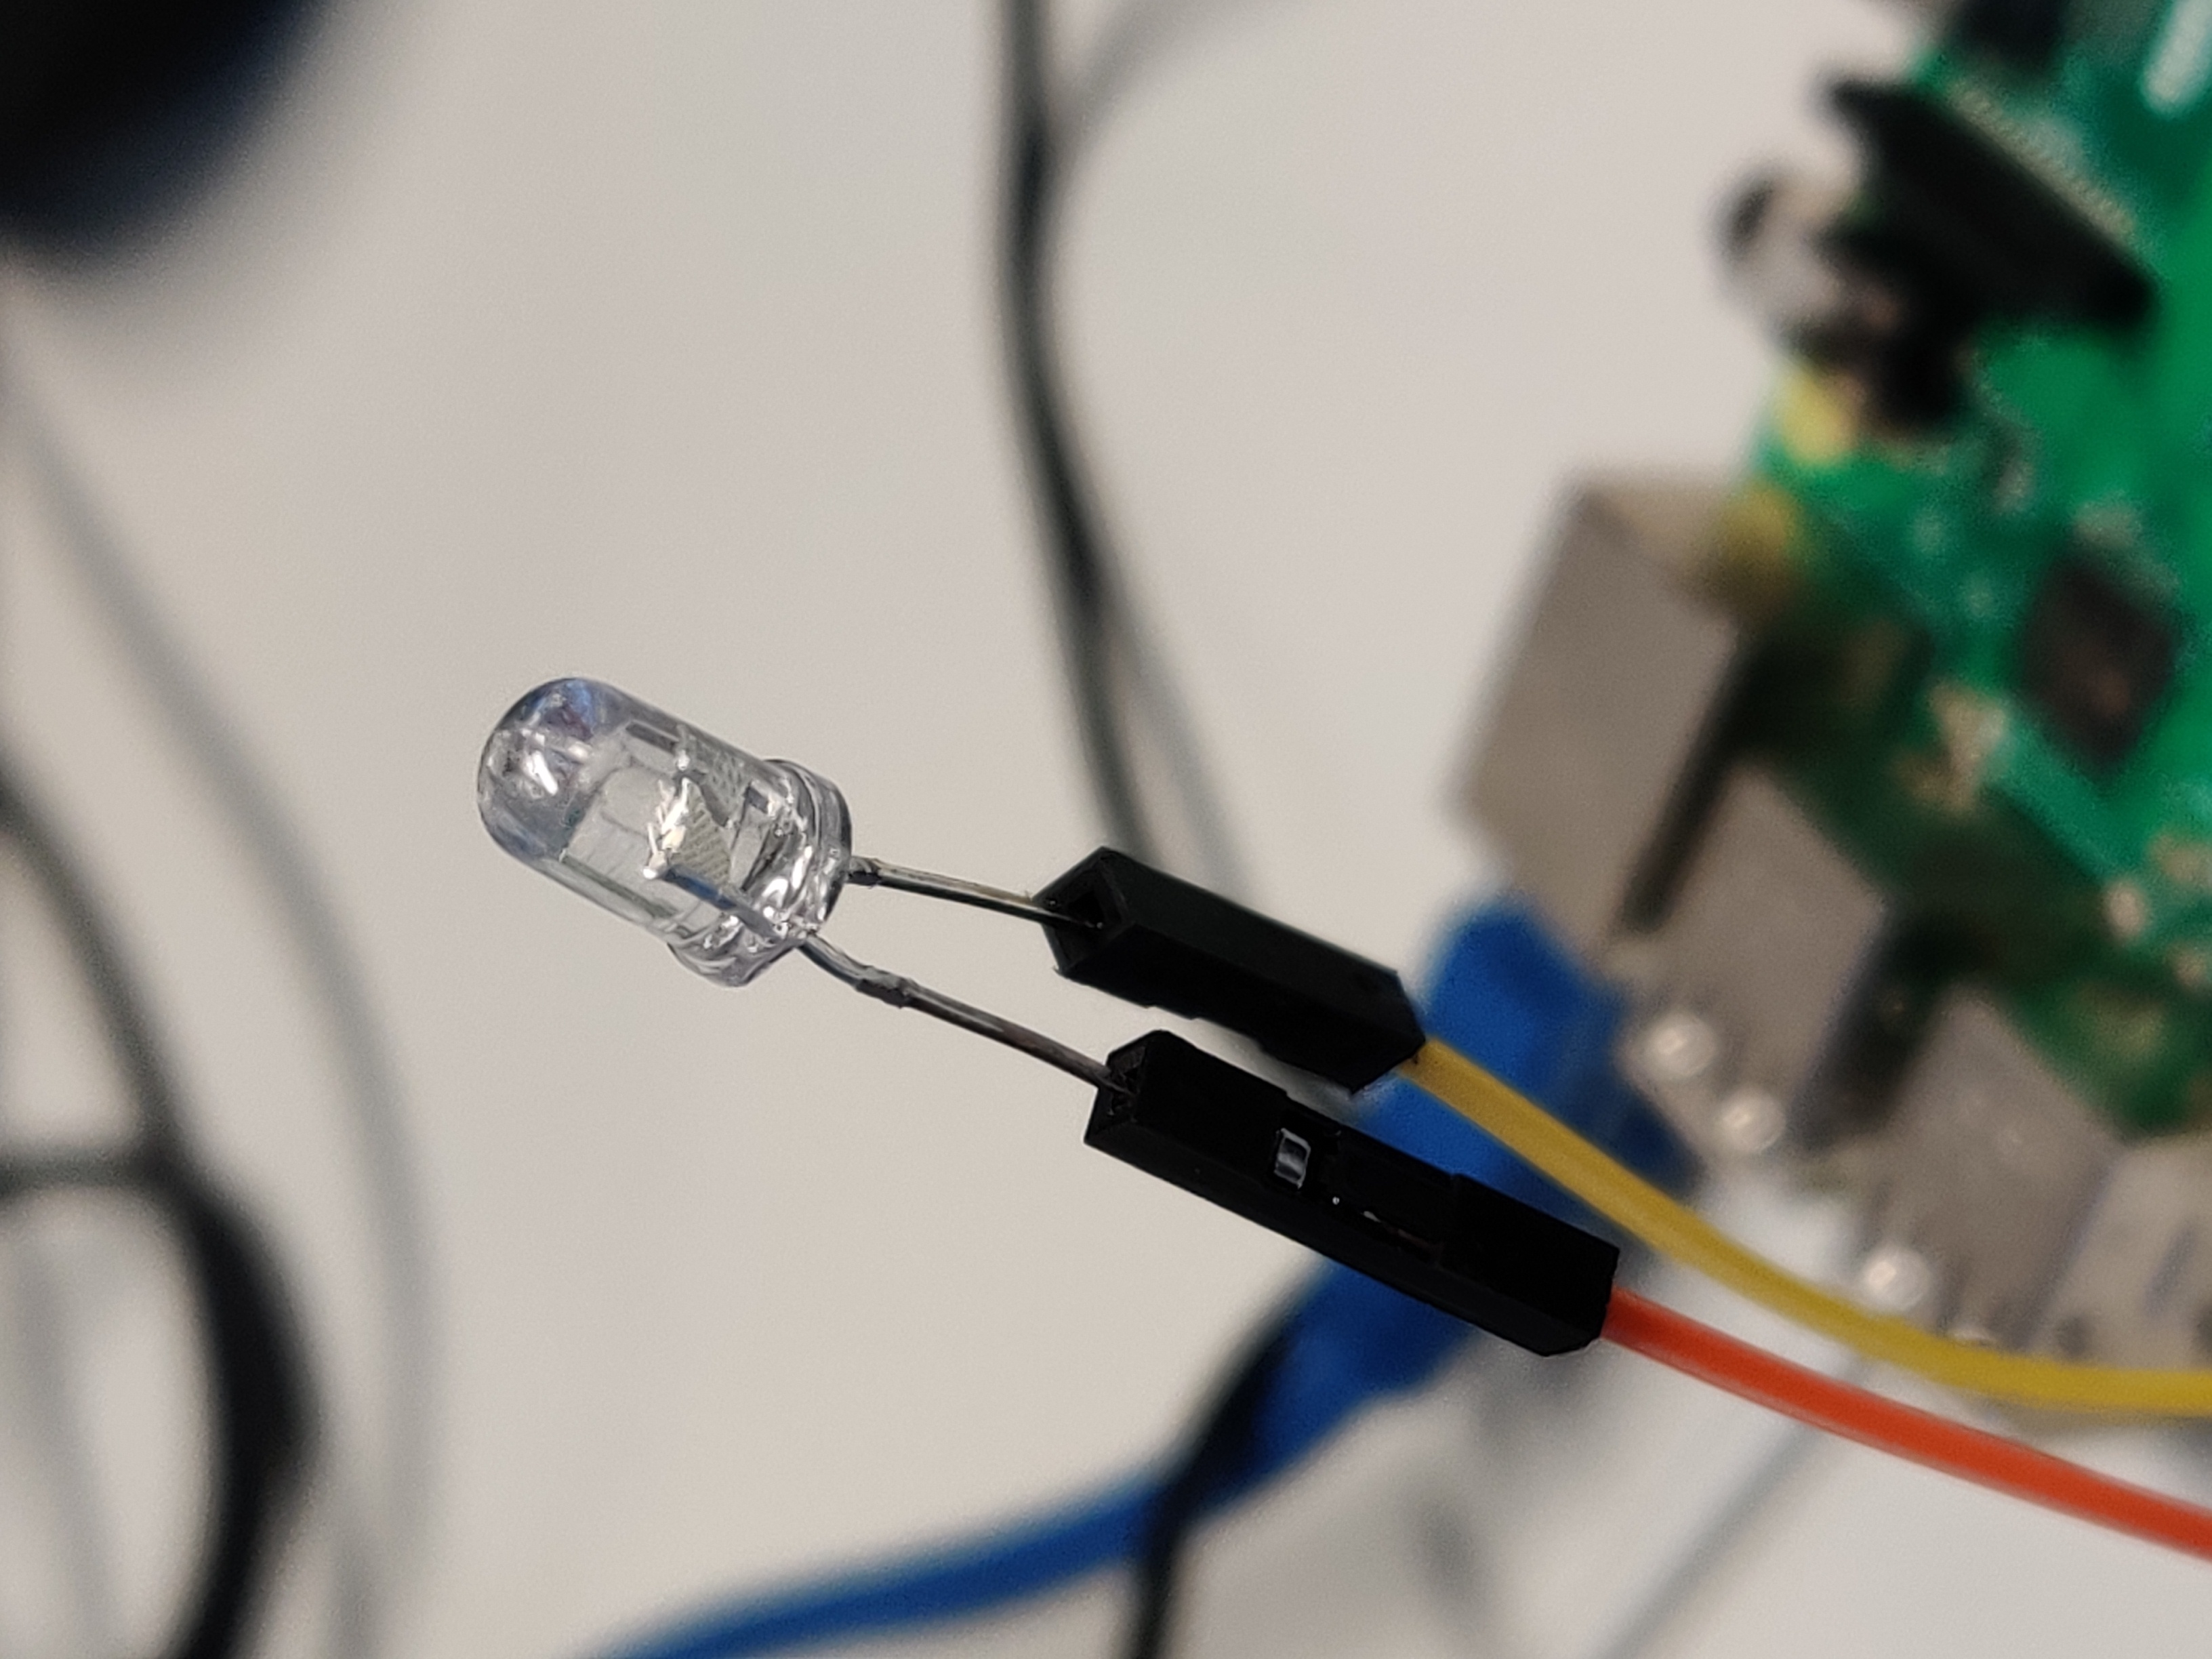
\includegraphics[width=0.8\textwidth]{images/ledOff}
	\caption{LED after alarm condition}
	\label{fig:images-ledOff}
\end{figure}

\subsubsection{Test 7: Square Wave Generator}

The Square Wave Generator function was written with a value of ``1'',
representing a frequency of 1Hz. Again this was visually verified. The flashing
LED cannot be demonstrated in the report.

\subsubsection{Test 8: Read Temperature}

The read temperature function prints the current temperature on the RTC, with a
precision of $\pm 0.25^{\circ}$C. This test outputs a value of $22^{\circ}$C.

\subsubsection{Test 9: Novel Function}

The novel function sets the RTC time and date to the system time and date, as
output from the Linux ``date'' utility. This was verified, as the output time
and date, as in Figure \ref{fig:images-testing}, were the current time and date
of execution of the program.
